\documentclass{standalone}
\usepackage{pgfplots}
\usepgfplotslibrary{groupplots,fillbetween}
\usepackage{animate}

\usepackage{pgf}
\usepackage{tikz}

\usetikzlibrary{fit}
\usetikzlibrary{positioning}
\usetikzlibrary{arrows}
\usetikzlibrary{automata}
\usetikzlibrary{backgrounds}
\usetikzlibrary{shapes.misc}

\begin{document}

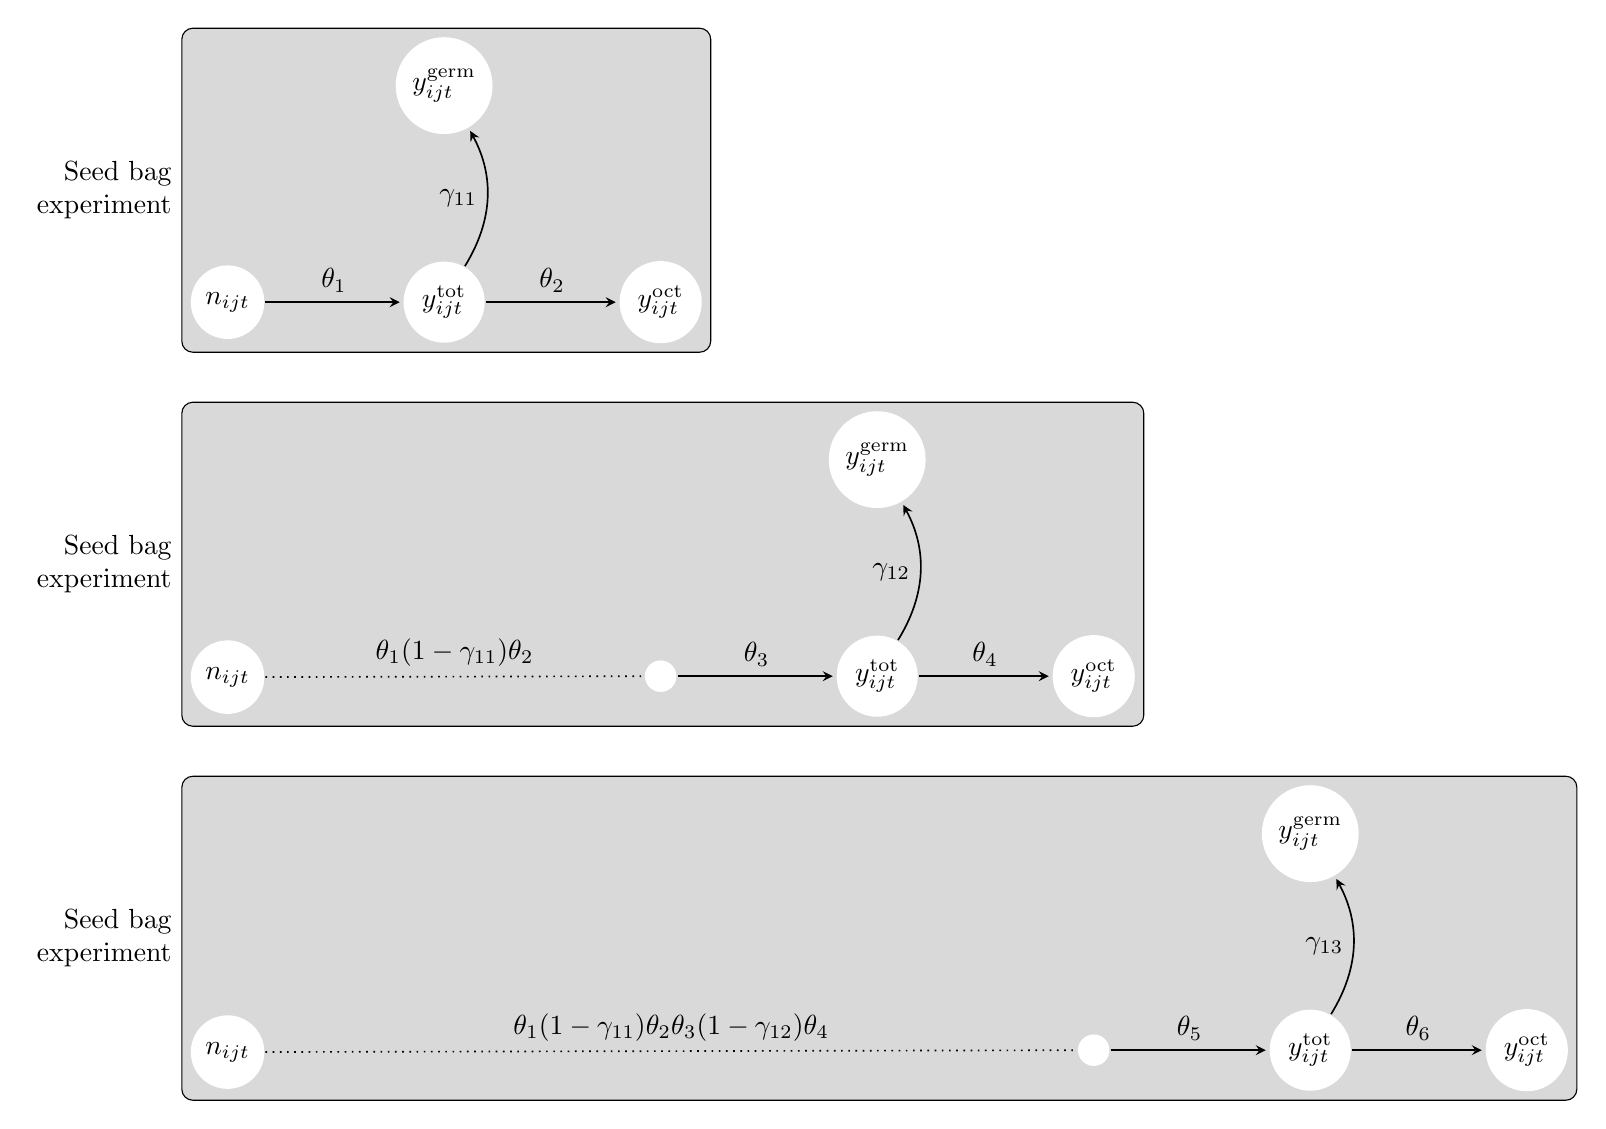
\begin{tikzpicture}[
            > = stealth, % arrow head style
            shorten > = 1pt, % don't touch arrow head to node
            auto,
            node distance = 2.75cm, % distance between nodes
            semithick % line style
        ]

        \tikzstyle{every state}=[
            draw = none,
            thick,
            fill = white,
            minimum size = 4mm
        ]

	% START OF SEED BAG EXPERIMENT
        \node[state] (N) [] {$n_{ijt}$};
        \node[state] (N2) [below = 3.8 cm of N] {$n_{ijt}$};
        \node[state] (N3) [below = 3.8 cm of N2] {$n_{ijt}$};

	% AGE 1 SEED BAG ESTIMATES      
        \node[state] (YJ) [right of=N] {$y^{\mathrm{tot}}_{ijt}$};
        \node[state] (YO) [right of=YJ] {$y^{\mathrm{oct}}_{ijt}$};
        \node[state] (G) [above of=YJ] {$y^{\mathrm{germ}}_{ijt}$};

        \path[->] (N) edge node {$\theta_1$} (YJ);
        \path[->] (YJ) edge node {$\theta_2$} (YO);
       	\path[->] (YJ) edge[bend right] node {$\gamma_{11}$} (G);

	% AGE 2 SEED BAG ESTIMATES      
        \node[state] (U2) [below = 4 cm of YO] {};
        \node[state] (YJ2) [right of=U2] {$y^{\mathrm{tot}}_{ijt}$};
        \node[state] (YO2) [right of=YJ2] {$y^{\mathrm{oct}}_{ijt}$};
        \node[state] (G2) [above of = YJ2] {$y^{\mathrm{germ}}_{ijt}$};

        \path[dotted,-] (N2) edge node {$\theta_1(1-\gamma_{11}) \theta_2 $} (U2);
        \path[->] (U2) edge node {$ \theta_3 $} (YJ2);
        \path[->] (YJ2) edge node {$\theta_4$} (YO2);
       	\path[->] (YJ2) edge[bend right] node {$\gamma_{12}$} (G2);

	% AGE 3 SEED BAG ESTIMATES      
        \node[state] (U3) [below  = 4 cm of YO2] {};
        \node[state] (YJ3) [right of=U3] {$y^{\mathrm{tot}}_{ijt}$};
        \node[state] (YO3) [right of=YJ3] {$y^{\mathrm{oct}}_{ijt}$};
        \node[state] (G3) [above of = YJ3] {$y^{\mathrm{germ}}_{ijt}$};

        \path[dotted,-] (N3) edge node {$\theta_1(1-\gamma_{11}) \theta_2 \theta_3 (1-\gamma_{12}) \theta_4  $} (U3);
        \path[->] (U3) edge node {$ \theta_5 $} (YJ3);
        \path[->] (YJ3) edge node {$\theta_6$} (YO3);
       	\path[->] (YJ3) edge[bend right] node {$\gamma_{13}$} (G3);


       	\begin{scope}[on background layer]
	\node[draw,fit=(N) (YJ) (YO) (G) , fill = gray!30, rounded corners, inner sep = .1cm, label={[label distance=0cm, align = right]left:{Seed bag \\ experiment}}] {};
	\node[draw,fit=(N2) (YJ2) (YO2) (G2) , fill = gray!30, rounded corners, inner sep = .1cm, label={[label distance=0cm, align = right]left:{Seed bag \\ experiment}}] {};
	\node[draw,fit=(N3) (YJ3) (YO3) (G3) , fill = gray!30, rounded corners, inner sep = .1cm, label={[label distance=0cm, align = right]left:{Seed bag \\ experiment}}] {};
	  \end{scope}

  \end{tikzpicture}
  
  \iffalse
  
   \node[state] (T1) [below right of=G] {$n^{\mathrm{gt}}_{ijt}$};
   	\path[dotted, ->] (Y2) edge node {} (T1);
        \node[state] (TG) [right of=T1] {$y^{\mathrm{gt}}_{ijt}$};
   	\path[->] (T1) edge node {$\theta_g$} (TG);
        \node[state] (T2) [below of=T1] {$n^{\mathrm{vt}}_{ijt}$};
   	\path[dotted, ->] (TG) edge node {} (T2);
        \node[state] (VG) [right of=T2] {$y^{\mathrm{vt}}_{ijt}$};
   	\path[->] (T2) edge node {$\theta_v$} (VG);
  	\node[draw,fit=(T1) (T2) (TG) (VG), label={[label distance=0cm, align = right]left:{Viability \\ trials}}] {};

  \fi
  
  \end{document}